\begin{figure}
\centering
\captionsetup{type=table}
\begin{small}
\begin{tabular}{lcccc}
\toprule
%  & \textbf{VAE} & \textbf{IWAE}& \textbf{WW} & \textbf{$\chi$-VAE} \\ \midrule
%  $\log p_\theta(X)$ & -17.37 & \textbf{-16.91} & -16.91 & -17.30\\
% IWELBO &  -17.37 & \textbf{-16.91} & -16.91 & -17.30\\
% \midrule
% PSIS & 0.57 & 0.25 & 0.53 & \textbf{0.04}\\
% $\norm{A}_2$ & 1.99 & \textbf{0.93} & 1.43 & 0.98 \\
% \midrule
% MAE & 7.71 & \textbf{2.41} & 2.70 & 7.14\\
& \textbf{VAE} & \textbf{IWAE} & \textbf{WW} & \textbf{$\rchi$-VAE}\\
\midrule
$\log p_\theta(X)$  & -17.65 & \textbf{-16.91} & -16.93 & -16.92\\
IWELBO  & -17.66 & \textbf{-16.92} & -16.96 & \textbf{-16.92}\\
\midrule
$\norm{A}_2$  & 1.69 & 1.30 & 2.32 & \textbf{1.13}\\
PSIS  & 0.54 & 0.53 & 0.66 & \textbf{0.47}\\
\midrule
% MAE  & 0.099 & \textbf{0.026} & 0.039 & 0.028\\
MAE  & 0.103 & 0.032 & 0.043 & \textbf{0.030}\\
\bottomrule
\end{tabular}
\end{small}
\caption[Results on the pPCA simulated data]{\label{table:mixture}Results on the pPCA simulated data. MAE refers to the mean absolute error in posterior expectation estimation.}

\end{figure}


\begin{figure}
\centering
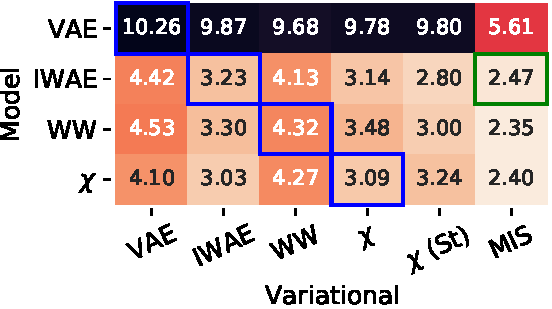
\includegraphics[width=0.4\textwidth]{figures/gaussian_l1_is_err_nu_cross.pdf}
\caption[MAE of posterior expectation estimation on pPCA for different methods]{MAE ($\times 10^2$) of posterior expectation estimation on pPCA for combinations of VAEs (row) and inference only (columns) frameworks. }\label{fig:pPCA-cross}
\end{figure}

\subsection{Experimental results}
\label{posterior_query}
We now investigate how well our understanding of EP, CHIVI, IWVI and VI may translate to WW, $\rchi$-VAE, IWAE, and the VAE. In particular, we generate synthetic data according to the pPCA model described in Eq.~\eqref{eq:lin_vae_gen} and assess how well these variants can estimate posterior expectations. We use a linear function for the mean and the log-variance of the variational distribution. This is a popular setup for approximate inference diagnostics~\cite{Turner2011} since the posterior has an analytic form, and the form is not typically a mean-field factorization. We propose a toy example of a posterior expectation, $\mathcal{Q}(f_\nu, x) = p_\theta(z_1 \geq \nu \mid x)$, obtained for $f_\nu(z) = \mathds{1}\{e_1^\top z \geq \nu\}$ with $e_1$ as the first vector of the canonical basis of $\mathbb{R}^d$. For this choice of $f_\nu$, the resulting posterior expectation is tractable since it is the cumulative density function of a Gaussian distribution. 
% Appendix~\ref{app:lin_gauss} contains further details for this experiment.

To evaluate the learned generative model, we provide goodness-of-fit metrics based on IWELBO on held-out data as well as the exact log-likelihood. In addition, we report the Pareto-smoothed importance sampling (PSIS) diagnostic \smash{$\hat{k}$} for assessing the quality of the variational distribution as a proposal~\cite{pmlr-v80-yao18a}. PSIS is computed by fitting a generalized Pareto distribution to the IS weights; it indicates the viability of the variational distribution for IS. For multiple importance sampling (MIS), we combine the proposal (learned on the same model) from IWAE, WW, and $\rchi$-VAE, as well as samples from the prior~\cite{hesterberg1995weighted} with equal weights.

When not stated otherwise, we report the median PSIS over $64$ observations, using $5,000$ samples from the posterior. %We use Adam~\cite{adam} for optimization of $\theta$ and $\phi$. 
We use $25$ particles (also for the VAE, as in~\cite{rainforth2018tighter}) per iteration for training the models, $10,000$ samples for reporting log-likelihood proxies and $200$ particles for making decisions. 
%We ran our experiments on a machine with a single NVIDIA GeForce RTX 2070 GPU. 
% I think it's potentially distracting to mention the hardware here---it doesn't really have any bearing on the results. --Jeff
All results are averaged across five random initializations of the neural network weights. 

Table~\ref{table:mixture} contains our results. IWAE, WW, and the $\rchi$-VAE outperform the VAE in terms of held-out exact likelihood (always close to the IWELBO). There is a slight preference for IWAE.
In terms of posterior approximation, we find that all algorithms yield a reasonable value for the PSIS diagnostic, in overall agreement with the spectral norm of $A$. PSIS values are not directly comparable between models, as they only measure the suitability of the variational distribution for a particular model. 
% As reported previously in~\cite{rainforth2018tighter}, the VAE learns a simpler model for which inference is easier. This explains the low values of PSIS for VAE.
% \jeff{Two sentences early we say PSIS aren't comparable across models, but here it sounds like we're comparing them across models.}
Finally, in terms of mean absolute error (MAE), IWAE and $\rchi$-VAE achieve the best result. For the VAE, the plugin estimator attains similar performance as the SNIS estimator.

In Figure~\ref{fig:pPCA-cross}, we fix these models and learn several proposal distributions for estimating the posterior expectations. We also report the PSIS values in Figure~\ref{fig:PCAPSIS}. For a fixed model, the proposal from the  $\rchi$-VAE often improves the MAE, and the one from MIS performs best. The three-step procedure (IWAE-MIS, shown in green) significantly improves on all of the single-proposal methods (shown in blue). The performance of WW when used to learn a proposal is not as good as expected. Better results may be found by increasing the number of particles or by using sleep phase updates~\cite{le2018revisiting}. With respect to the $\rchi$-VAE, we noticed that replacing the Gaussian distribution as the variational distribution with a Student-t distribution usually improves the MAE. 
As the heavier tails of the Student-t distribution also help to avoid an infinite $\rchi^2$ divergence, we systematically use it in the $\rchi$-VAE for the real-world applications.

\begin{figure}
    \centering
    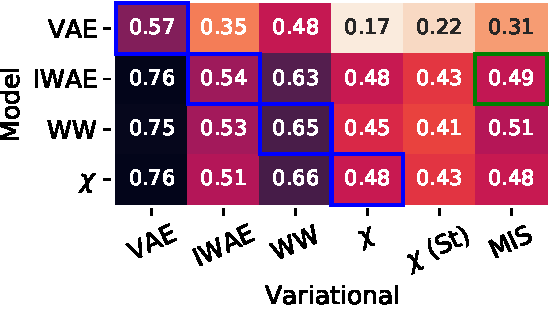
\includegraphics[width=0.4\textwidth]{figures/gaussian_other_cross.pdf}
    \caption[PSIS metric for pPCA]{
    PSIS for pPCA: combinations of VAEs (row) and inference only (columns) frameworks. 
    }
    \label{fig:PCAPSIS}
\end{figure}
